\documentclass[twoside]{article}

\usepackage{aistats2026}
% Submission: anonymous (default). Camera-ready: \usepackage[accepted]{aistats2026}.

\usepackage[utf8]{inputenc}
\usepackage[T1]{fontenc}
\usepackage[round]{natbib}
\renewcommand{\bibname}{References}
\renewcommand{\bibsection}{\subsubsection*{\bibname}}
\usepackage{amsmath,amssymb}
\usepackage{booktabs}
\usepackage{graphicx}
\usepackage{xcolor}
\usepackage[colorlinks=true,allcolors=black]{hyperref}
\usepackage{url}
\graphicspath{{figures/}}

\begin{document}

\runningtitle{Latent-Source Identifiability from Observational Neural Recordings Is Not Confirmable}

\twocolumn[
\aistatstitle{Latent-Source Identifiability from Observational Neural Recordings\\ Is Not Confirmable}
\aistatsauthor{Anonymous Authors}
\aistatsaddress{Anonymous Institution}
]

\begin{abstract}
Recovering the hidden causes of a measured signal from the signal alone is the promise behind causal representation learning, and its identifiability theorems state when that promise holds: under certain assumptions, the latent sources of an observed mixture are recovered up to ordering, sign and scale.
Brain recordings are where this promise matters most, and components recovered from observational recordings are routinely reported as latent sources.
We ask against what such a claim is checked.
No observational recording carries a reference for its latent sources that is independent of the method; the claim can be refuted, when a necessary condition of the theorem fails in the data, but it cannot be confirmed.
We make this concrete on scalp EEG.
We build a benchmark whose sources are known by construction, a recurrent generator trained on EEG and stressed along the axes that distinguish EEG from idealised mixing, and evaluate six unsupervised methods against a measured chance level and a subspace reference.
With the sources known, each identifiability route has an EEG nuisance that satisfies its objective without carrying the sources: slow drift for segment-based methods, $1/f$ autocorrelation for dependence-based ones.
With the sources unknown, no quantity a practitioner can compute has a stable relation to recovery.
On real EEG the checkable rank condition holds, so the claim is not refuted; scored against the experimental cue, the only reference the recording offers, the segment-based method's components carry no more of it than the components of methods that never use the segments.
Identifiability claims on observational recordings therefore require a ground-truth benchmark with the stresses of the modality or an experimental manipulation.
\end{abstract}

\section{Introduction}
\label{sec:intro}

Two people speak at a party and two microphones record; each microphone hears a mixture of both voices.
Recovering the speakers from the mixtures is the canonical motivation of blind source separation, and independent component analysis (ICA), nonlinear ICA and causal representation learning have formalised the conditions under which it is possible \citep{hyvarinen2000ica,hyvarinen1999nonlinear,hyvarinen2016tcl,khemakhem2020ivae,scholkopf2021toward,kugelgen2023nonparametric}.
Under those conditions the latent sources are \textit{identifiable} from the observations up to ordering, sign and scale.
The same intuition has been carried into neuroscience: a scalp electrode hears a mixture of many cortical and non-cortical sources, and a method that unmixes the recording into interpretable components is read as recovering something close to the generators of cognition \citep{makeig1996ica,michel2019eeg,hyvarinen2016tcl,halva2021snica}.

\begin{figure*}[t]
  \centering
  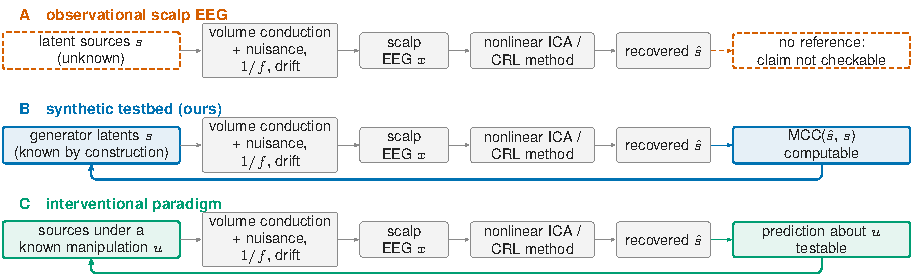
\includegraphics[width=0.9\textwidth]{fig0_concept.pdf}
  \caption{Three routes to a latent-source claim. (A) On an observational recording the recovered components $\hat{s}$ can be compared to nothing that is independent of the method; inverse solutions, decoders and concurrent recordings each encode a model of their own. (B) A benchmark whose sources are known by construction closes the loop with a computable recovery score. (C) An experimental manipulation $u$ (a cue, a stimulation, a closed-loop task) yields a prediction that the recovered components must satisfy.}
  \label{fig:concept}
\end{figure*}

In this work we ask a question that this practice leaves open: when an identifiability method is applied to an observational recording and a set of recovered sources is reported, against what is the claim checked?
The party analogy assumes a listener who can hear one speaker at a time.
For the brain no such listener exists.
Source reconstructions encode their own model, decoders return a function of the components together with the decoder, and no recording modality provides the latent sources themselves (Figure~\ref{fig:concept}A).
The identifiability claim is therefore in an unusual position.
It can be \textit{refuted}: every identifiability theorem has necessary conditions on the data, and some of them can be checked on the recording.
However, it cannot be \textit{confirmed}: a method that satisfies its own objective may have done so on a nuisance that carries none of the sources, and nothing in the recording distinguishes the two cases.

We make this position concrete on scalp electroencephalography (EEG), the modality where the problem is most acute (many sources, few channels, a strong nonstationary background) and for which nonlinear-ICA identifiability methods have been proposed on non-invasive recordings \citep{hyvarinen2016tcl,halva2021snica}.
Our contributions are the following.
\begin{itemize}\setlength{\itemsep}{1pt}
  \item A benchmark whose sources are known by construction: a recurrent generator trained on EEG, mixed into synthetic recordings and stressed along five axes that distinguish EEG from the idealised mixing problem; every score comes with a measured chance level and a subspace reference (Section~\ref{sec:benchmark}).
  \item With the sources known, each identifiability route has an EEG nuisance that satisfies its objective without carrying the sources, slow drift for segment-based methods and $1/f$ autocorrelation for dependence-based ones; a modulation shared by all sources and a source count near the channel count defeat every method (Section~\ref{sec:truth}, Figure~\ref{fig:axes}).
  \item With the sources unknown, no quantity a practitioner can compute has a stable relation to recovery; the accuracy the methods themselves report rises exactly where recovery falls (Section~\ref{sec:blind}, Figure~\ref{fig:diag}).
  \item On real EEG the checkable rank condition holds, so the claim is not refuted; scored against the experimental cue, the only reference the recording offers, the segment-based method's components carry no more of it than the components of methods that never use the segments (Section~\ref{sec:real}, Figure~\ref{fig:real}).
\end{itemize}
Taken together, these results support one requirement: an identifiability claim on observational recordings should be accompanied by a benchmark with the stresses of the modality, or by an experimental manipulation that yields a testable prediction (Figure~\ref{fig:concept}B,C).

\section{Refutable, not confirmable}
\label{sec:argument}

A scalp recording at $D$ electrodes is a projection of far more cortical and non-cortical current sources, smeared by volume conduction \citep{nunez2006electric,michel2019eeg}.
For any observed $x$, infinitely many source configurations are compatible with it, and source-localisation methods restore uniqueness only relative to a chosen prior.
Testing a recovery therefore needs a reference that is independent of the method.
The candidates on an observational recording are inverse solutions, behavioural decoding and concurrent recordings in another modality, and each encodes a model of its own: agreement between two model-based unmixings shows that the two models agree, a decoder absorbs any error in the components that is consistent with the readout, and intracranial contacts index cortical patches rather than the latent sources a nonlinear-ICA theorem speaks about.
A component set that scores well on any of these can be a faithful recovery, a confound or a self-consistent artefact.

The theorems nevertheless leave something testable.
Time-contrastive learning (TCL; \citealp{hyvarinen2016tcl}) requires that the segment-wise modulation of the sources spans the source space, i.e.\ that the modulation matrix has full column rank (Appendix~\ref{app:tcl}); iVAE \citep{khemakhem2020ivae} requires the analogous invertibility for its auxiliary variable; for second-order linear separation the exact condition is that no two sources have proportional variance profiles \citep{pham2001blind,kleinsteuber2013uniqueness}; permutation-contrastive learning (PCL; \citealp{hyvarinen2017pcl}) requires non-Gaussian innovations.
If all sources always get louder together, the modulation matrix has rank one and only the total power is identified (Appendix~\ref{app:tcl}).
This is visible in the segment covariances of the recording itself, with no ground truth, and it refutes the claim.
What no recording can supply is the converse.
A segment classifier that predicts segment identity from slow drift, or a contrastive objective fed by the autocorrelation of $1/f$ noise, satisfies the method's objective as well as the sources would, and the recording offers no quantity that separates the two.
This is Popper's asymmetry in its original form, data can refute a hypothesis but cannot verify it \citep{popper1959logic}, applied to a claim that is routinely reported as verified.
The rest of the paper measures both halves.

\section{Related work}
\label{sec:related}

\paragraph{How identifiability methods are validated on brain recordings.}
TCL was introduced on MEG and validated by decoding the stimulus modality from its features \citep{hyvarinen2016tcl}; later nonlinear-ICA applications to MEG validate in the same way, by downstream classification \citep{halva2021snica,zhu2023unsupervised}.
Decoding is route C of Figure~\ref{fig:concept}, and we use it ourselves in Section~\ref{sec:real}; the point of Sections~\ref{sec:argument} and \ref{sec:blind} is that it is necessary and not sufficient, since the decoder absorbs whatever error in the components is consistent with the label, and that it is the only one of the usual checks that does not share a model with the method.
The nonlinear-ICA papers also validate on synthetic sources \citep{hyvarinen2016tcl,khemakhem2020ivae}, with generic sources and mixing; what those benchmarks lack is the nuisance structure of the modality, which is what breaks the objectives here.

\paragraph{Ground-truth EEG simulation.}
Simulated EEG with known sources is established in the source-localisation and connectivity literature: SEREEGA \citep{krol2018sereega}, EEGSourceSim \citep{barzegaran2019eegsourcesim}, neural-mass models \citep{jansen1995electroencephalogram} and pseudo-EEG connectivity benchmarks \citep{haufe2019simulation}.
These generators place known sources through a forward model; none varies the quantities an identifiability objective depends on (the segment-wise modulation, its rank and magnitude, drift relative to the segment rate), and none reports a chance level or a subspace reference for a recovery score.
The benchmark of Section~\ref{sec:benchmark} adds these, and a physics leadfield in place of its learned mixing reproduces its orderings (Appendix~\ref{app:robust}).

\paragraph{Plausibility checks in EEG practice.}
The ICA-on-EEG literature judges components by dipolarity \citep{delorme2012dipolar}, test-retest reliability and physiological plausibility.
Each is a model of what a source should look like rather than a reference for what it is; Section~\ref{sec:blind} measures the analogous diagnostics, run-to-run and split-half agreement, against known recovery.

\paragraph{Identifiability theory.}
\citet{locatello2019challenging} showed that unsupervised disentanglement is impossible without inductive bias or supervision; the auxiliary-variable theorems \citep{hyvarinen2016tcl,hyvarinen2019auxiliary,khemakhem2020ivae} and interventional results \citep{kugelgen2023nonparametric} supply that structure as a property of the data.
Our question is downstream of theirs: whether that property holds on a given observational recording can be refuted but not confirmed, and we measure both halves on EEG.

\section{A benchmark with known sources}
\label{sec:benchmark}

\paragraph{Generator.}
We train a shallow piecewise-linear recurrent neural network (shPLRNN; \citealp{brenner2024shPLRNN,hess2023gtf}) on the 22-channel BCI Competition IV-2a EEG \citep{brunner2008bci,tangermann2012review}, with $M$ latent states and a learned linear observation model $x = Wz$.
The trained model is used strictly as a generator, in the sense of a formal surrogate of the system it was fitted to \citep{durstewitz2023reconstructing}, the use that recurrent latent-dynamics models of neural recordings are built for \citep{pandarinath2018lfads,koppe2019identifying,ramezanian2022generative}: its stochastic free run is the ground-truth source signal $s$ and its $W$ the mixing.
One generator is trained per source count $M \in \{2, 4, 8, 16, 22, 32\}$; the clean operating point is $M = 4$ sources in $D = 22$ channels.
Training on EEG supplies the mixing geometry (a learned $22 \times M$ observation matrix whose conditioning grows with $M$), a latent dimensionality per $M$ and process noise calibrated on the recordings; the stochastic free run is spectrally flatter than the latents the model encodes from EEG, and Appendix~\ref{app:realism} reruns the benchmark with a recipe whose free run matches the EEG spectrum.
Every cell draws a training and a held-out trajectory of $T = 2000$ samples (8~s at 250~Hz, cut into 20 segments of 0.4~s) from the same generator; methods are fit on the first and scored on the second (Appendix~\ref{app:protocol}).

\paragraph{Stresses.}
Each axis violates one assumption in a controlled way, harder to the right in Figure~\ref{fig:axes}: (a) a $1/f$ background, the aperiodic component of every EEG spectrum \citep{donoghue2020parameterizing}, at decreasing signal-to-noise ratio; (b) a pointwise nonlinearity after mixing; (c) first-order coupling between the sources; (d) the diversity of the segment-wise modulation, from each source following its own variance profile to one gain shared by all; (e) the number of sources against the fixed channel count, past the point where sources outnumber channels.
Axis (d) is parametrised by an observable quantity, the \textit{co-modulation fraction}: the fraction of the segment-to-segment change of the channel covariance that follows a single spatial pattern (Appendix~\ref{app:placement}).
It can be computed on any recording, which is what lets real EEG be placed on the axis in Section~\ref{sec:real}.

\paragraph{Methods.}
PCA and FastICA \citep{hyvarinen1999fastica} are the linear baselines; FastICA is the positive control for linear mixing of independent sources.
TCL and iVAE identify through segment-wise nonstationarity, PCL through temporal dependence, and CEBRA \citep{schneider2023cebra} is a current neural-data method whose time-contrastive objective likewise rests on local temporal structure.
All methods receive the same 20 segments and return $M$ components; the iVAE is trained on per-channel standardised inputs with the evidence lower bound under a unit-variance Gaussian likelihood.
Implementation details are given in Appendix~\ref{app:methods}.

\paragraph{Scores and references.}
Methods that return source estimates are scored by the mean correlation with the signed sources after each component is matched to its best source (MCC; \citealp{hyvarinen2016tcl,khemakhem2020ivae}).
TCL and CEBRA return energy-like features (features that track the power of a source rather than its signed waveform), since under variance modulation TCL identifies $s^2$ up to a linear map (Appendix~\ref{app:tcl}); they are scored by the canonical-correlation MCC against $|s|$ (which is unchanged by any linear map of the features), and the two scores are read within a row of Figure~\ref{fig:axes}, never across.
Two references accompany every score.
The \textit{chance band} is the 95th percentile of the score of surrogate components that are statistically matched to the sources but independent of them, measured per cell.
The \textit{rotation reference} is the score of the true sources under a random rotation, i.e.\ of a method that recovers the source subspace but does not separate it; a permutation MCC at that level is subspace recovery, not identification (Appendix~\ref{app:scores}).
Error bars throughout are bootstrap 95\% intervals over seeds.

\section{With the sources known}
\label{sec:truth}

\begin{figure*}[t]
  \centering
  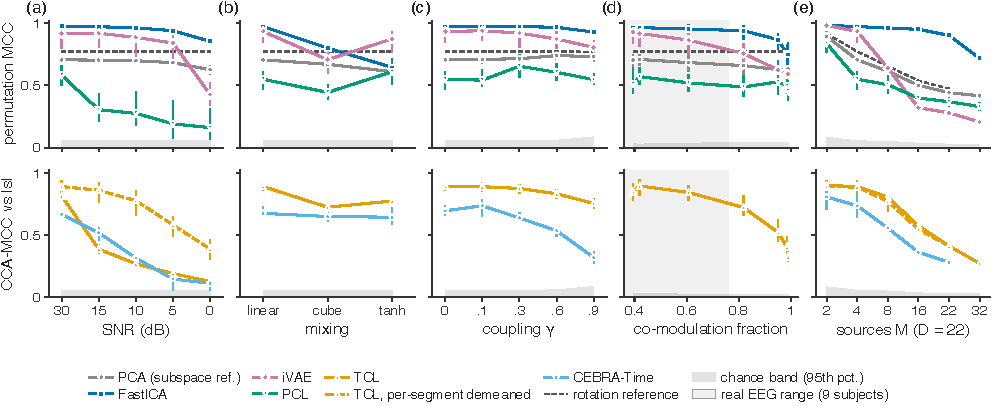
\includegraphics[width=\textwidth]{fig1_axes.pdf}
  \caption{Held-out recovery along five EEG-relevant stress axes; harder to the right in every panel. Top row: permutation MCC against the signed sources (PCA, FastICA, iVAE, PCL), with the rotation reference (dashed), the score of a method that recovers the source subspace but not the sources. Bottom row: linear-invariant CCA-MCC against $|s|$ for the energy-like features of TCL, TCL after per-segment demeaning of the observations (dashed) and CEBRA-Time. Grey band: measured chance level (95th percentile of surrogate components). Error bars: bootstrap 95\% intervals over 20 seeds (PCA, FastICA, TCL), 5 seeds (iVAE, PCL, demeaned TCL, panel d, $M=32$) or 3 seeds (CEBRA). (a) $1/f$ background; (b) pointwise mixing nonlinearity; (c) first-order source coupling; (d) co-modulation fraction of the segment-wise modulation, from source-specific profiles to a single shared gain, with the range of nine BCI IV-2a subjects shaded; (e) number of sources against 22 channels, each $M$ with its own trained generator and learned mixing. Numbers in Table~\ref{tab:full}.}
  \label{fig:axes}
\end{figure*}

Figure~\ref{fig:axes} and Table~\ref{tab:full} give the result.
On clean linear mixing every method except PCA recovers the sources; PCA sits on the rotation reference everywhere, it finds the subspace and never separates it, which is why it serves as the subspace reference.
Pointwise nonlinearity and source coupling, the two axes closest to the classical theory, cost the nonlinear methods little.
The breaks are elsewhere, and each has a mechanism.

\paragraph{Drift feeds the segment classifier.}
As the $1/f$ background grows, TCL falls to the chance band while FastICA is barely affected (Figure~\ref{fig:axes}a).
The failure is not noise as such.
Power below the segment rate shifts the mean of each segment, the classifier learns segment identity from those shifts, and its features track drift rather than source variance; removing the per-segment mean of the observations restores TCL to its clean level down to 10~dB (dashed line, Appendix~\ref{app:robust}).
PCL fails from the other side: $1/f$ noise is temporally dependent, so it feeds a dependence-based objective, and PCL's own pair-discrimination accuracy rises along the axis while its recovery falls.
CEBRA, whose positive pairs are short time offsets, inherits TCL's profile without any labels.

\paragraph{A shared modulation identifies only total power.}
Along axis (d) every nonlinear method declines as the co-modulation fraction approaches one, TCL to the level the rank argument of Appendix~\ref{app:tcl} predicts: with one shared profile the modulation matrix has rank one, only $\|s\|^2$ is identified, and the individual sources collapse while the group energy is still decoded from the features (Appendix~\ref{app:robust}).
FastICA degrades too, since a common gain makes near-Gaussian sources spherically symmetric.
More data does not move these cells, nor the stationary one; the failure is in the assumption, not in the sample (Figure~\ref{fig:robust}b).
The ordering holds down to the modulation magnitudes of real EEG at second-scale segmentation (Figure~\ref{fig:real}a).

\paragraph{Sources against channels.}
As $M$ approaches $D$ the nonlinear methods fall towards the rotation reference, and past $D$ every method falls (Figure~\ref{fig:axes}e).
For TCL this is a finite-sample failure: with sixteen times more data its score at $M = D$ rises to that of the clean cell (Figure~\ref{fig:robust}b).
For the linear methods the limit is physical rather than statistical: a sphere-model leadfield in place of the learned mixing reproduces every ordering of Figure~\ref{fig:axes} and steepens this decline through its conditioning (Figure~\ref{fig:robust}d, Appendix~\ref{app:robust}).

\section{With the sources unknown}
\label{sec:blind}

\begin{figure*}[t]
  \centering
  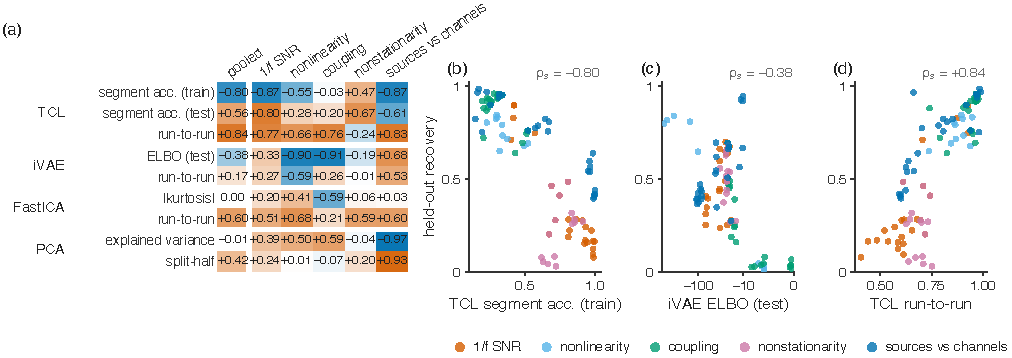
\includegraphics[width=\textwidth]{fig2_diagnostics.pdf}
  \caption{What a practitioner can compute without ground truth, against what the benchmark knows. (a) Spearman correlation between an observational diagnostic of the fitted model and its true held-out recovery, pooled over the cells of Figure~\ref{fig:axes} and within each stress axis; blue negative, orange positive. (b--d) Three of those diagnostics against true recovery, one point per (axis, condition, seed) cell, coloured by axis: TCL's training segment accuracy, the iVAE evidence lower bound, and the agreement between two TCL fits on the same data.}
  \label{fig:diag}
\end{figure*}

A practitioner has none of Figure~\ref{fig:axes}.
What they have is the fitted model: TCL's segment-classification accuracy, the iVAE's evidence lower bound, the agreement between two fits, the non-Gaussianity of FastICA's components, the explained variance of PCA.
Figure~\ref{fig:diag} correlates each of these with the true held-out recovery across the cells of the benchmark, pooled and within each axis.
No diagnostic keeps a stable relation to recovery.
The accuracy that TCL papers report is anti-diagnostic in training: it is highest where recovery is lowest, because drift is easier to classify than source variance (Figure~\ref{fig:diag}b).
The iVAE's bound tracks recovery on the coupling axis and anti-tracks it on the source-count axis (Figure~\ref{fig:diag}c).
Run-to-run agreement, the best pooled diagnostic, is uninformative inside the nonstationarity axis, where the real nuisance lives (Figure~\ref{fig:diag}d); an iVAE that is consistently wrong is consistent.
The sign of every column of Figure~\ref{fig:diag}a depends on which stress the data happen to carry, so calibrating any of these diagnostics requires the benchmark, and the calibration flips across the stresses that a real recording mixes.
This is the second half of Section~\ref{sec:argument} as a measurement.

\section{Real scalp EEG}
\label{sec:real}

\begin{figure*}[t]
  \centering
  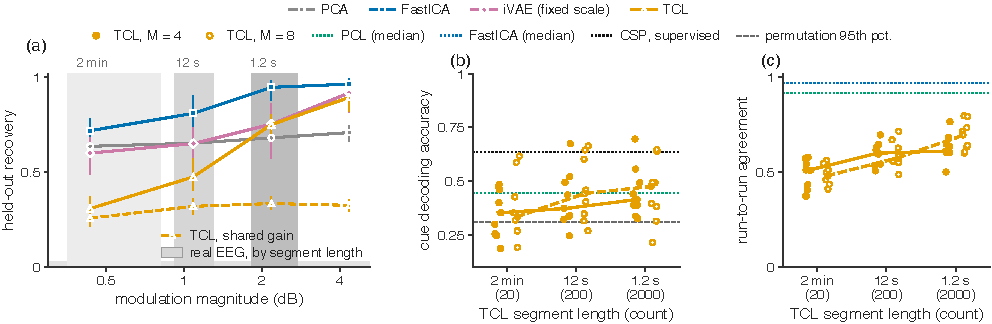
\includegraphics[width=\textwidth]{fig3_real_eeg.pdf}
  \caption{Real EEG against the benchmark. (a) Held-out recovery against the magnitude of the segment-wise modulation (standard deviation of the per-segment log-variance, in dB; log axis) for the source-specific schedule, and for TCL under one shared gain (dashed); chance band in grey; mean and bootstrap 95\% interval over 5 seeds. Shaded: the range of the nine BCI IV-2a subjects' observed modulation magnitude when the recording is cut into 20, 200 or 2000 segments (2~min, 12~s, 1.2~s per segment). (b) Four-class cue decoding accuracy from the per-trial log-variance of TCL components fit without labels on three runs and scored on the other three, against TCL's segment length; one point per subject, lines at the median, filled $M = 4$, hollow $M = 8$. Dotted: medians of PCL, which does not use segments, and of supervised CSP on all 22 channels; dashed: label-permutation 95th percentile. (c) Agreement between TCL fits on different runs, with the PCL and FastICA medians. Protocols in Appendix~\ref{app:real}.}
  \label{fig:real}
\end{figure*}

Two things can be done with the recording itself: check the conditions the theorems make checkable, and score the components against the one reference the experiment provides.

\paragraph{Real EEG is in the regime where the benchmark's conclusions hold.}
Two properties of the segment-wise modulation are observable without ground truth: how much of it follows one spatial pattern (the co-modulation fraction of Section~\ref{sec:benchmark}) and how large it is (the standard deviation of the per-segment log-variance).
On the nine BCI IV-2a subjects the co-modulation fraction lies in the left half of axis (d) of Figure~\ref{fig:axes}, in the broad band as in the motor band, away from the shared-gain regime (Table~\ref{tab:mod}); the rank condition is not refuted.
The magnitude depends on how the recording is segmented.
Figure~\ref{fig:real}a repeats the modulation cells of the benchmark at smaller magnitudes and marks where the subjects fall when their recordings are cut into 20, 200 or 2000 segments.
At the second-scale segmentation that TCL's own protocol uses, the magnitude of real EEG's modulation is the magnitude at which every conclusion of Section~\ref{sec:truth} holds, including the shared-gain failure; the benchmark cells use 20 segments of 0.4~s, so the segment length is comparable and the recordings supply many more segments.
At minute-scale segments the modulation is too weak for any segment-based method, which is a property of the segmentation rather than of the recording.
A TCL recovery reported on these recordings at its natural segment length would therefore pass every check the recording allows, and the failures that remain are the ones that cannot be seen in the recovery: drift, which preprocessing can remove but no score reveals, and nuisance processes with a spatial pattern of their own (Appendix~\ref{app:robust}).

\paragraph{The cue is a reference, and the components barely carry it.}
BCI IV-2a has an experimental manipulation: a randomised four-class motor-imagery cue with a known cortical locus.
We fit each unsupervised method on three runs of a subject without labels and score its components on the other three by how well their per-trial log-variance decodes the cue (Appendix~\ref{app:cue}); a label-permutation null and a supervised ceiling, common spatial patterns (CSP), bracket the result.
Figure~\ref{fig:real}b,c follow TCL across the same three segment lengths; the other methods do not use segments and enter as reference lines.
Finer segments help TCL, as panel (a) predicts: its decoding accuracy and its agreement between fits on different runs both rise.
At its natural segment length, however, TCL's components decode the cue no better than the components of methods that never use the segments (paired Wilcoxon tests over the nine subjects against PCA, FastICA and PCL, none significant; Appendix~\ref{app:cue}), well below CSP ($p = 0.004$), and at every segment length they remain the least reproducible of the unsupervised methods ($p = 0.004$ against each).
On real EEG the segment-based method, at its best setting, finds nothing about the only available reference that a linear baseline does not.

\section{Discussion}
\label{sec:discussion}

The asymmetry of Section~\ref{sec:argument} is not specific to EEG: no observational recording carries a reference for its latent sources that is independent of the method used to recover them.
What is specific to a modality is the set of nuisances that satisfy an identifiability objective without carrying the sources, and a benchmark has to contain them.
Synthetic benchmarks are already the unit of empirical claim in disentanglement and nonlinear ICA \citep{locatello2019challenging,hyvarinen2016tcl,khemakhem2020ivae}; what the standard generators lack are the stresses of the modality.
For scalp EEG and MEG, which share the same geometry (far fewer channels than sources) and the same nonstationary background, these are drift below the segment rate, $1/f$ autocorrelation, co-modulation of all sources and a source count beyond the channel count.
The benchmark of Section~\ref{sec:benchmark} varies each of them, and its conclusions are unchanged when the generator is retrained to reproduce the spectrum of real EEG (Appendix~\ref{app:realism}).

In light of this, an identifiability claim on observational recordings should come with one of two things.
Either a recovery score on a benchmark with the stresses of the modality, reported next to a measured chance level and a subspace reference, as in Figure~\ref{fig:axes}; or an experimental manipulation that yields a prediction the recovered components must satisfy, as in Figure~\ref{fig:real}b.
Both are available today; the cue test above uses a public dataset and no new recording.
The methods themselves remain useful for denoising, dimensionality reduction and feature extraction, and none of these uses needs an identifiability claim; directed-interaction analyses between recovered components \citep{granger1969investigating,seth2015granger,nolte2008meg} do, since what a Granger test on $\hat{s}$ identifies depends on what $\hat{s}$ is \citep{stokes2017study}.
What changes is the claim that is admissible: not that the latent sources were recovered, but that a stated condition was not refuted, or that a stated prediction was met.


\section*{AI Use Statement}
A large language model (Anthropic Claude, through Claude Code) assisted this work as an editorial and coding assistant: it drafted candidate text from the authors' notes and results, which the authors revised; it tightened prose; and it wrote and refactored analysis and plotting code under the authors' direction.
The position, the experimental design, the execution and interpretation of every experiment, the figures and every decision about content are the authors'.
Every model-generated change was reviewed by the authors before inclusion.

\acknowledgments{This work is supported by IVADO. We thank Guillaume Dumas, Pooneh Mousavi, Dhanya Sridhar and Irina Rish for helpful discussions. This research was enabled in part by compute resources provided by Mila (\url{https://mila.quebec}) and the Digital Research Alliance of Canada (\url{https://alliancecan.ca}). The implementation and writing was assisted by AI. M.R-P.\ is fully responsible for the scientific content and integrity of this paper.}

\bibliographystyle{plainnat}
\bibliography{references}

\section*{Checklist}

\begin{enumerate}

  \item For all models and algorithms presented, check if you include:
  \begin{enumerate}
    \item A clear description of the mathematical setting, assumptions, algorithm, and/or model. [Yes] Sections~\ref{sec:argument}--\ref{sec:benchmark}, Appendices~\ref{app:protocol}--\ref{app:scores} and \ref{app:tcl}.
    \item An analysis of the properties and complexity (time, space, sample size) of any algorithm. [Not Applicable] No new algorithm is proposed; the sample-size dependence of the evaluated methods is reported in Appendix~\ref{app:robust}.
    \item (Optional) Anonymized source code, with specification of all dependencies, including external libraries. [Yes] Supplementary material.
  \end{enumerate}

  \item For any theoretical claim, check if you include:
  \begin{enumerate}
    \item Statements of the full set of assumptions of all theoretical results. [Yes] Appendix~\ref{app:tcl} restates the assumptions of the TCL identifiability theorem used in Section~\ref{sec:argument}.
    \item Complete proofs of all theoretical results. [Not Applicable] No new theorem is claimed; the rank consequence in Appendix~\ref{app:tcl} follows directly from the cited result.
    \item Clear explanations of any assumptions. [Yes] Appendix~\ref{app:tcl}.
  \end{enumerate}

  \item For all figures and tables that present empirical results, check if you include:
  \begin{enumerate}
    \item The code, data, and instructions needed to reproduce the main experimental results (either in the supplemental material or as a URL). [Yes] Supplementary material; the EEG data are the public BCI Competition IV-2a set.
    \item All the training details (e.g., data splits, hyperparameters, how they were chosen). [Yes] Appendices~\ref{app:protocol}, \ref{app:methods} and \ref{app:real}.
    \item A clear definition of the specific measure or statistics and error bars (e.g., with respect to the random seed after running experiments multiple times). [Yes] Section~\ref{sec:benchmark} and Appendix~\ref{app:scores}; every figure caption states the seeds and the interval.
    \item A description of the computing infrastructure used. (e.g., type of GPUs, internal cluster, or cloud provider). [Yes] Appendix~\ref{app:methods}.
  \end{enumerate}

  \item If you are using existing assets (e.g., code, data, models) or curating/releasing new assets, check if you include:
  \begin{enumerate}
    \item Citations of the creator If your work uses existing assets. [Yes] BCI Competition IV-2a \citep{brunner2008bci,tangermann2012review}; shPLRNN \citep{brenner2024shPLRNN,hess2023gtf}; CEBRA \citep{schneider2023cebra}; MNE \citep{gramfort2014mne}.
    \item The license information of the assets, if applicable. [Yes] Stated in the supplementary material.
    \item New assets either in the supplemental material or as a URL, if applicable. [Yes] Benchmark code and trained generators in the supplementary material.
    \item Information about consent from data providers/curators. [Not Applicable] Public benchmark dataset.
    \item Discussion of sensible content if applicable, e.g., personally identifiable information or offensive content. [Not Applicable]
  \end{enumerate}

  \item If you used crowdsourcing or conducted research with human subjects, check if you include:
  \begin{enumerate}
    \item The full text of instructions given to participants and screenshots. [Not Applicable]
    \item Descriptions of potential participant risks, with links to Institutional Review Board (IRB) approvals if applicable. [Not Applicable]
    \item The estimated hourly wage paid to participants and the total amount spent on participant compensation. [Not Applicable]
  \end{enumerate}

\end{enumerate}


\appendix
\onecolumn
\aistatstitle{Latent-Source Identifiability from Observational Neural Recordings Is Not Confirmable:\\ Supplementary Materials}
\section{Generator and evaluation protocol}
\label{app:protocol}

\paragraph{Data.}
BCI Competition IV-2a \citep{brunner2008bci,tangermann2012review}: nine subjects, four-class motor imagery, 22 EEG channels at 250~Hz.
The recordings are cut into 750-sample windows, giving 2592 trials, which are the units of the hierarchical generator.

\paragraph{Generator training.}
A shallow piecewise-linear recurrent neural network \citep{brenner2024shPLRNN} with $M$ latent states, hidden width 20 and a linear observation model $x = Wz$, $W \in \mathbb{R}^{22 \times M}$, is trained with generalised teacher forcing \citep{hess2023gtf} (learning rate $10^{-4}$ for the shared parameters and $10^{-3}$ for the trial-specific ones, batch size 64, sequence length 50, 500 epochs).
One generator is trained per $M \in \{2, 4, 8, 16, 22, 32\}$ with the same recipe, and each supplies its own $W$.

\paragraph{Source trajectories.}
The deterministic free run of a trained generator contracts to a fixed point, so the sources are its stochastic free run $z_t = f(z_{t-1}) + \epsilon_t$, $\epsilon_t \sim \mathcal{N}(0, \mathrm{diag}(\sigma^2))$, where $\sigma$ is the per-latent median of the generator's one-step prediction residual over all 2592 training trials.
Each seed draws one trial's parameters and starts from that trial's first real frame; 500 burn-in steps are discarded, $T = 2000$ steps are kept, each latent is standardised to unit variance (the scores are invariant to this), the sources are projected through $W$ and the configured nuisance is added.

\paragraph{Held-out protocol.}
For every cell two trajectories are drawn from the same generator with the same trial parameters and initial frame (generator seeds $s$ and $s + 50000$).
One draw of the condition randomness (segment-wise modulation gains, coupling matrix, $W$, noise type and noise power, the latter set from the training trajectory's clean signal power) is applied to both.
The training trajectory is standardised with its own statistics and the test trajectory with the training statistics.
Every method is fit on the training trajectory and applied to the test one; permutation matching and the canonical-correlation map are fit on the training trajectory and applied unchanged to the test one.

\paragraph{Segments and modulation.}
The $T = 2000$ steps are cut into 20 equal segments, which are the labels given to TCL, iVAE and segment-conditioned CEBRA.
Unless the modulation axis says otherwise, each source is rescaled per segment by an independent $\mathrm{Exp}(1)$ variance (source-specific profiles).
Along axis (d) the per-source log-variance profile is $((1-a)\,g_0 + a\,g_i)/\sqrt{(1-a)^2 + a^2}$ with $g_0$ a profile common to all sources and $g_i$ a source-specific one, for $a \in \{1, 0.75, 0.5, 0.35, 0.2, 0.1, 0\}$; $a = 1$ is the source-specific law and $a = 0$ a single shared gain (rank-one modulation matrix).
Cells with $r \in \{1, 2, 3, 4\}$ distinct profiles shared among the four sources fall on the same curve (Table~\ref{tab:mod}).

\paragraph{Other axes.}
Pink noise is generated by filtering Gaussian white noise with a $1/f$ amplitude spectrum and scaled to the configured signal-to-noise ratio ($\{30, 15, 10, 5, 0\}$~dB); the remaining axes use 20~dB Gaussian sensor noise.
Mixing nonlinearity applies $\phi \in \{\mathrm{id},\, x \mapsto x^3,\, \tanh\}$ pointwise after $W$.
Source coupling applies $z_t \leftarrow (1-\gamma)\, z_t + \gamma\, A z_{t-1}$ with $A$ a fixed random matrix of unit spectral norm, $\gamma \in \{0, 0.1, 0.3, 0.6, 0.9\}$, after the segment rescaling and before mixing.
At $M = 32 > D$ the linear methods return 22 components and are scored over the 22 matched pairs.

\paragraph{Seeds.}
Twenty seeds for PCA, FastICA and TCL; five for iVAE, PCL, demeaned TCL, axis (d) and $M = 32$; three for CEBRA.
Each seed draws a different trial's generator parameters and a different fitting seed.

\section{Methods and implementation}
\label{app:methods}

\paragraph{PCA, FastICA.} \texttt{scikit-learn} with default tolerances, $M$ components.
\paragraph{TCL.} Per-timestep MLP feature extractor (three layers, hidden width 64, LeakyReLU) and a multinomial logistic regression over the 20 segments; Adam, learning rate $10^{-3}$, 200 epochs; the $M$-dimensional features are the components \citep{hyvarinen2016tcl}.
\textit{Demeaned TCL} removes the per-segment, per-channel mean from the training and the test observations before fitting; this removes only power below the segment rate and keeps 91\% of the source power.
\paragraph{iVAE.} Encoder and decoder MLPs (three layers, hidden width 64), a conditional Gaussian prior factorised over latent dimensions with the segment index as auxiliary variable, per-channel standardised inputs and the evidence lower bound under a unit-variance Gaussian likelihood; Adam, 200 epochs; the posterior mean is the component \citep{khemakhem2020ivae}.
\paragraph{PCL.} The TCL encoder with the per-component dependence model of \citet{hyvarinen2017pcl}, trained for 200 epochs to discriminate consecutive pairs $(x_t, x_{t-1})$ from time-permuted pairs; scored like the source-estimating methods.
PCL has no positive control on the generator's sources, whose innovations are Gaussian; on AR(1) sources with Laplacian innovations the same implementation scores 0.88 (stationary) and 0.90 (modulated), on Gaussian AR(1) sources 0.71, the rotation level.
\paragraph{CEBRA.} CEBRA 0.6.1 \citep{schneider2023cebra}, per-timestep MLP with a Euclidean (non-normalised) output of dimension $M$, 500 iterations, time-contrastive positives at offsets up to 10 samples (CEBRA-Time).
In every cell its features are energy-like (canonical correlation with $|s|$ well above that with $s$), so they are scored as TCL's.
A segment-conditioned variant gives the same profile.
\paragraph{Hardware.} All fits run on CPU (Apple M4); generator training on Apple MPS.

\section{Scores, chance level and rotation reference}
\label{app:scores}

\paragraph{Permutation MCC.} Mean absolute correlation between components and signed sources after solving the linear assignment problem on the absolute correlation matrix \citep{hyvarinen2016tcl}; the assignment is fit on the training trajectory.
\paragraph{Linear-invariant MCC.} Under segment-wise variance modulation of Gaussian sources the sufficient statistic is $q(s) = s^2$, and TCL identifies $q(s)$ only up to a linear map (Appendix~\ref{app:tcl}).
TCL and CEBRA are therefore scored by the mean canonical correlation between their features and $|s|$, with the canonical map fit on the training trajectory.
$|s|$ is a lighter-tailed monotone surrogate of $s^2$; scoring against $s^2$ instead lowers the values by $0.01$--$0.08$ without changing which conditions recover and which fail (Table~\ref{tab:mod}, last column).
\paragraph{Chance level.} Both scores are maximised over a matching, so an estimator carrying no information does not score zero.
For each cell the true sources are drawn as in the sweep and scored against surrogate components that are statistically matched to them but independent of them: an independent draw from the same generator, and a circular time shift of the sources themselves, which preserves every autocorrelation and destroys only the alignment.
The band in the figures is the 95th percentile over 20 surrogate repeats, maximised over both constructions and both scores.
\paragraph{Rotation reference.} The permutation MCC of the true sources under a Haar-random orthogonal rotation (20 repeats, same matching): $0.92$, $0.77$, $0.66$, $0.54$ and $0.47$ at $M = 2, 4, 8, 16, 22$.
A method that recovers the source subspace without separating it scores at this level; it is specific to each $M$ and to the sources' correlation structure, and it does not apply to the linear-invariant score, which is unchanged by any rotation.

\section{Full results}
\label{app:tables}

\begin{table}[h]\centering\small
\caption{Held-out recovery on the benchmark of Figure~\ref{fig:axes}. PCA, FastICA and TCL: mean over 20 seeds with bootstrap 95\% interval; iVAE, PCL and demeaned TCL: mean over 5 seeds. Permutation MCC against the signed sources for PCA, FastICA, iVAE and PCL (rotation reference in the last column); CCA-MCC against $|s|$ for TCL. Null: 95th percentile of the chance level over surrogate constructions and scores. The modulation block was run at 15~dB $1/f$, so its source-specific cell is the 15~dB cell of the first block; the modulation axis of Figure~\ref{fig:axes}d at the clean operating point is in Table~\ref{tab:mod}.}
\label{tab:full}
\begin{tabular}{llcccccccc}\toprule
axis & cell & PCA & FastICA & iVAE & PCL & TCL & TCL demeaned & null & rotation \\ \midrule
$1/f$ SNR (dB) & 30 & 0.71 [0.68, 0.74] & 0.98 [0.96, 0.99] & 0.92 & 0.58 & 0.81 [0.78, 0.84] & 0.89 & 0.05 & 0.77 \\
 & 15 & 0.70 [0.68, 0.73] & 0.97 [0.96, 0.98] & 0.92 & 0.31 & 0.39 [0.35, 0.43] & 0.86 & 0.05 & 0.77 \\
 & 10 & 0.70 [0.67, 0.73] & 0.96 [0.95, 0.98] & 0.89 & 0.28 & 0.27 [0.24, 0.29] & 0.78 & 0.05 & 0.77 \\
 & 5 & 0.68 [0.66, 0.71] & 0.94 [0.92, 0.95] & 0.84 & 0.19 & 0.19 [0.17, 0.21] & 0.58 & 0.05 & 0.77 \\
 & 0 & 0.63 [0.59, 0.66] & 0.86 [0.83, 0.88] & 0.43 & 0.16 & 0.13 [0.11, 0.14] & 0.39 & 0.05 & 0.77 \\
\midrule
mixing & linear & 0.71 [0.68, 0.74] & 0.97 [0.96, 0.99] & 0.93 & 0.55 & 0.89 [0.85, 0.92] & -- & 0.05 & 0.77 \\
 & cube & 0.67 [0.62, 0.72] & 0.80 [0.79, 0.82] & 0.71 & 0.44 & 0.72 [0.70, 0.75] & -- & 0.05 & 0.77 \\
 & tanh & 0.61 [0.59, 0.63] & 0.64 [0.63, 0.66] & 0.87 & 0.61 & 0.77 [0.74, 0.80] & -- & 0.05 & 0.77 \\
\midrule
coupling $\gamma$ & 0.0 & 0.71 [0.68, 0.74] & 0.97 [0.96, 0.99] & 0.93 & 0.55 & 0.89 [0.85, 0.92] & -- & 0.05 & 0.77 \\
 & 0.1 & 0.71 [0.68, 0.74] & 0.97 [0.96, 0.99] & 0.94 & 0.54 & 0.89 [0.85, 0.92] & -- & 0.05 & 0.77 \\
 & 0.3 & 0.72 [0.68, 0.75] & 0.97 [0.96, 0.98] & 0.92 & 0.65 & 0.87 [0.84, 0.91] & -- & 0.06 & 0.77 \\
 & 0.6 & 0.74 [0.71, 0.78] & 0.97 [0.96, 0.98] & 0.87 & 0.61 & 0.83 [0.79, 0.87] & -- & 0.06 & 0.77 \\
 & 0.9 & 0.73 [0.69, 0.77] & 0.93 [0.91, 0.95] & 0.81 & 0.55 & 0.75 [0.71, 0.79] & -- & 0.09 & 0.77 \\
\midrule
modulation (15~dB $1/f$) & source-specific & 0.70 [0.68, 0.73] & 0.97 [0.96, 0.98] & 0.92 & 0.31 & 0.39 [0.35, 0.43] & 0.86 & 0.05 & 0.77 \\
 & shared gain & 0.66 [0.64, 0.68] & 0.79 [0.76, 0.82] & 0.61 & 0.29 & 0.28 [0.27, 0.29] & 0.33 & 0.04 & 0.78 \\
 & none (stationary) & 0.64 [0.61, 0.66] & 0.72 [0.68, 0.76] & 0.59 & 0.36 & 0.05 [0.05, 0.06] & 0.17 & 0.06 & 0.78 \\
\midrule
$M$ ($D = 22$) & 2 & 0.90 [0.85, 0.93] & 0.98 [0.98, 0.99] & 0.98 & 0.84 & 0.90 [0.85, 0.94] & 0.89 & 0.08 & 0.92 \\
 & 4 & 0.71 [0.68, 0.74] & 0.97 [0.96, 0.99] & 0.93 & 0.55 & 0.89 [0.85, 0.92] & 0.89 & 0.05 & 0.77 \\
 & 8 & 0.61 [0.60, 0.63] & 0.96 [0.95, 0.97] & 0.64 & 0.51 & 0.81 [0.79, 0.82] & 0.77 & 0.05 & 0.66 \\
 & 16 & 0.50 [0.49, 0.51] & 0.95 [0.94, 0.96] & 0.32 & 0.40 & 0.57 [0.56, 0.58] & 0.55 & 0.03 & 0.54 \\
 & 22 & 0.44 [0.43, 0.45] & 0.90 [0.88, 0.92] & 0.28 & 0.37 & 0.41 [0.41, 0.42] & 0.41 & 0.03 & 0.47 \\
\bottomrule
\end{tabular}
\end{table}

\begin{table}[h]\centering\small
\caption{Modulation-diversity axis (Figure~\ref{fig:axes}d and Figure~\ref{fig:real}a; $M = 4$, 20~dB Gaussian noise, 5 seeds): held-out recovery against the observed co-modulation fraction of the segment-wise modulation. $a$ is the source-specific weight of the profile, $r$ the number of distinct profiles. The nine BCI IV-2a subjects have shares of 0.22--0.76 at 1--40~Hz and 0.24--0.42 at 8--30~Hz.}
\label{tab:mod}
\begin{tabular}{lcccccccc}\toprule
cell & co-modulation fraction & rank & PCA & FastICA & iVAE & PCL & TCL & TCL vs $s^2$ \\ \midrule
$a = 1$ & 0.42 & 4 & 0.71 & 0.97 & 0.92 & 0.57 & 0.89 & 0.81 \\
$a = 0.75$ & 0.39 & 4 & 0.70 & 0.96 & 0.93 & 0.51 & 0.85 & 0.78 \\
$a = 0.5$ & 0.61 & 4 & 0.68 & 0.95 & 0.86 & 0.52 & 0.84 & 0.78 \\
$a = 0.35$ & 0.82 & 4 & 0.66 & 0.94 & 0.76 & 0.49 & 0.72 & 0.67 \\
$a = 0.2$ & 0.95 & 4 & 0.63 & 0.87 & 0.62 & 0.53 & 0.52 & 0.50 \\
$a = 0.1$ & 0.99 & 4 & 0.63 & 0.75 & 0.59 & 0.49 & 0.40 & 0.38 \\
$a = 0$ & 0.99 & 1 & 0.64 & 0.75 & 0.59 & 0.46 & 0.32 & 0.31 \\
$r = 3$ & 0.59 & 3 & 0.69 & 0.89 & 0.81 & 0.47 & 0.74 & 0.68 \\
$r = 2$ & 0.63 & 2 & 0.66 & 0.89 & 0.72 & 0.45 & 0.53 & 0.48 \\
$r = 1$ & 0.99 & 1 & 0.64 & 0.74 & 0.58 & 0.45 & 0.35 & 0.32 \\
\bottomrule\end{tabular}\end{table}

\section{Robustness of the benchmark}
\label{app:robust}

\begin{figure}[h]
  \centering
  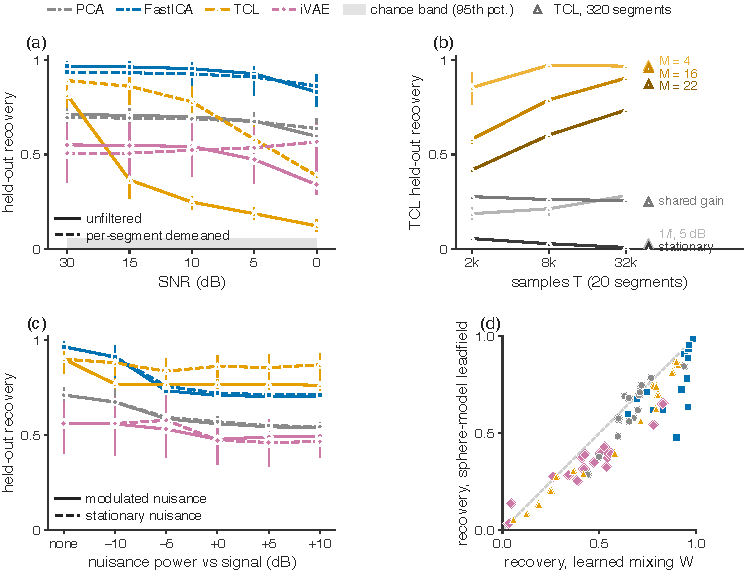
\includegraphics[width=0.78\textwidth]{figR_robustness.pdf}
  \caption{Robustness of Figure~\ref{fig:axes}. (a) Held-out recovery against the $1/f$ signal-to-noise ratio without preprocessing (solid) and after per-segment demeaning of the observations (dashed). (b) TCL against the length $T$ of the training trajectory at the stressed cells, 20 segments (lines) and 320 segments at $T = 32000$ (hollow). (c) Recovery with an additional nuisance component that is not among the sources, at $-10$ to $+10$~dB relative to the signal, with its variance modulated across segments like the sources' (solid) or constant (dashed). (d) Recovery with a sphere-model leadfield in place of the learned mixing, one point per cell of Figure~\ref{fig:axes}. Means over 5 seeds, bootstrap 95\% intervals.}
  \label{fig:robust}
\end{figure}

\paragraph{Preprocessing.}
Removing the per-segment mean of the observations restores TCL on the $1/f$ axis to its clean level down to 10~dB and leaves the other methods within a few hundredths of their values (Figure~\ref{fig:robust}a); its held-out segment accuracy rises at the same time, showing that the classifier had been fitting drift.
Zero-phase high-pass filters at one to four times the segment rate have the same effect on TCL and remove 18--35\% of the source power, which costs the other methods.
The shared-gain and stationary cells stay failed after any preprocessing.

\paragraph{Data quantity.}
With the same generator and mixing, TCL's score at $M = 22$ rises monotonically with the length of the training trajectory and with the number of segments, up to the clean level at $T = 32000$ with 320 segments (Figure~\ref{fig:robust}b); the linear methods are already saturated.
The shared-gain and stationary cells do not move with data, as the rank argument predicts, and the $1/f$ cells become worse with more segments, which give the classifier more drift signatures to memorise.

\paragraph{Group energy under shared profiles.}
With $r$ distinct modulation profiles shared among the four sources, the energies $\sum_{i \in g} s_i^2$ of the groups sharing a profile are decoded from the frozen TCL features with held-out $R^2$ above $0.8$ at every $r$, while the squares of individual sources within a group are decoded only up to the ceiling implied by the rotation ambiguity; rank deficiency coarsens the identified statistics to the invariants of the ambiguity group rather than destroying them.

\paragraph{Nuisance component.}
One additional white Gaussian signal on a random unit-norm spatial pattern, not among the sources, costs TCL about $0.13$ as soon as its variance is modulated across segments, already at a tenth of the signal power and no more at ten times it: one of TCL's features tracks the nuisance envelope (Figure~\ref{fig:robust}c).
A stationary nuisance of the same power costs TCL $0.02$--$0.06$.
The other methods lose one component to the nuisance once its power exceeds $-5$~dB, independent of modulation.

\paragraph{Leadfield.}
Replacing the learned $W$ by a physics leadfield (MNE three-layer sphere model fitted to the 22 BCI IV-2a electrodes \citep{gramfort2014mne}, $M$ current dipoles at random positions and orientations, rescaled to the learned $W$'s mean row norm) reproduces the ordering of every axis of Figure~\ref{fig:axes} (Figure~\ref{fig:robust}d).
The leadfield's condition number is $10^3$ at $M = 16$ and $10^4$ at $M = 22$, so the decline with $M$ is steeper for every method than with the learned mixing.

\paragraph{Capacity.}
A TCL network with four times the hidden width or five times the epochs changes the stressed cells by at most $0.04$ and lowers the clean cell, so the reported setting is the strongest of those tested.

\section{Generator realism}
\label{app:realism}

\begin{figure}[h]
  \centering
  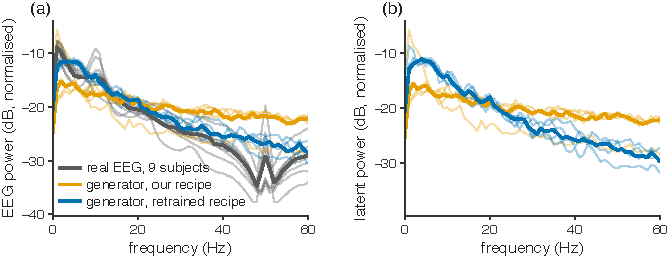
\includegraphics[width=0.6\textwidth]{figA_generator_realism.pdf}
  \caption{(a) Normalised power spectra of real BCI IV-2a EEG (per subject) and of the generator's synthetic EEG $Wz$ (per seed) for the recipe of Appendix~\ref{app:protocol} and for a recipe with a generalised-teacher-forcing floor of $0.2$ and hidden width 64; (b) the corresponding latent spectra. Thin lines: individual subjects or seeds; thick: median.}
  \label{fig:realism}
\end{figure}

The latents that the generator encodes from real EEG have a $1/f$ spectrum with an alpha peak; its stochastic free run under the recipe of Appendix~\ref{app:protocol} is flatter (Figure~\ref{fig:realism}).
Training with a generalised-teacher-forcing floor of $0.2$ and hidden width 64 gives free runs whose spectral slope, alpha excess and lag-one autocorrelation match the encoded latents.
Rerunning the full benchmark on generators trained with this recipe reproduces Figure~\ref{fig:axes} qualitatively (Figure~\ref{fig:axes_realistic}): TCL fails on the stationary and shared-gain cells and recovers along the $1/f$ axis only after demeaning, PCL survives the stationary cell, and every method falls with $M$.
These sources are more strongly inter-correlated than the main benchmark's, so the rotation reference and the chance band are higher at $M = 4$ (0.83 and 0.13), and the free runs are EEG-like for $M \le 8$.

\begin{figure}[h]
  \centering
  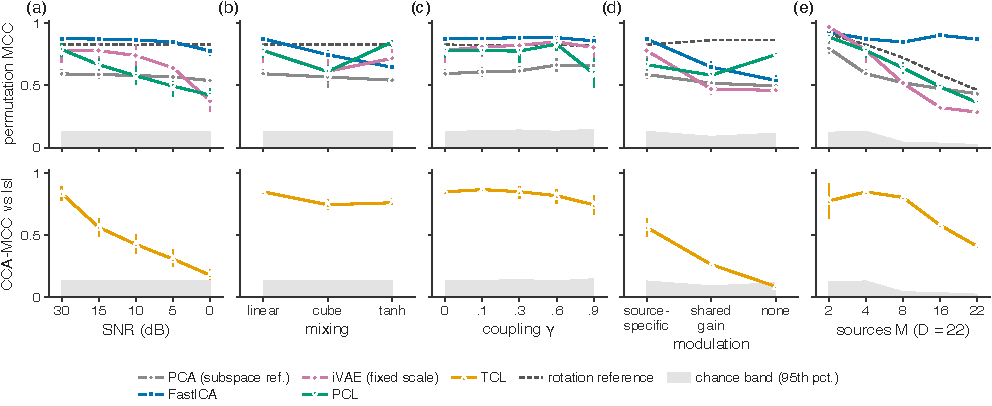
\includegraphics[width=\textwidth]{fig1_axes_realistic.pdf}
  \caption{Figure~\ref{fig:axes} on the generators of Appendix~\ref{app:realism} (5 seeds; panel (d) uses the three categorical modulation cells).}
  \label{fig:axes_realistic}
\end{figure}

\section{Real-EEG protocols}
\label{app:real}

\subsection{Observable properties of the segment-wise modulation}
\label{app:placement}
\paragraph{Co-modulation fraction.}
The recording is cut into the 20 contiguous segments TCL uses.
Each segment's channel covariance is whitened by the mean covariance and mapped to the tangent space by the matrix logarithm; the 20 tangent vectors are centred and their singular values taken.
The co-modulation fraction is the fraction of the segment-to-segment change that follows the dominant pattern, after subtracting the mean spectrum of 20 stationary surrogates (multivariate phase randomisations of the whole recording, which keep every auto- and cross-spectrum and remove the nonstationarity).
A single shared profile gives a share of one.
The statistic is computed identically on every synthetic cell of axis (d) and on the nine BCI IV-2a subjects (all six motor-imagery runs, 22 channels, 1--40~Hz and 8--30~Hz).
Real subjects have shares of 0.22--0.76 (median 0.39) at 1--40~Hz and 0.24--0.42 (median 0.32) at 8--30~Hz; on the benchmark TCL falls below $0.5$ only at shares of $0.95$ and above.

\paragraph{Magnitude.}
The magnitude of the modulation is the standard deviation, across segments and components, of the per-segment log-variance in dB.
On the benchmark it is the nominal standard deviation of the log-variance profile: $4.3$~dB for the $\mathrm{Exp}(1)$ law of the main sweep, and $2.2$, $1.1$ and $0.4$~dB for the cells of Figure~\ref{fig:real}a, obtained by scaling the log-variance profiles by $0.5$, $0.25$ and $0.1$ with everything else unchanged (Table~\ref{tab:mag}).
On real EEG it is computed on four FastICA components of the 1--40~Hz recording of each subject, cut into 20, 200 or 2000 contiguous segments, with the estimation floor (the same statistic on white noise of the same length) removed in quadrature; the two sides measure the same quantity with different estimators.
Across the nine subjects the median magnitude is $0.4$, $1.0$ and $2.0$~dB at 20, 200 and 2000 segments.

\begin{table}[h]\centering\small
\caption{Held-out recovery against the magnitude of the segment-wise modulation ($M = 4$, 20~dB Gaussian noise, 5 seeds; Figure~\ref{fig:real}a). Source-specific profiles ($a = 1$) for all methods; TCL also at $a = 0.5$ and under one shared gain ($a = 0$).}
\label{tab:mag}
\begin{tabular}{lcccccc}\toprule
magnitude (dB) & PCA & FastICA & iVAE & TCL & TCL, $a = 0.5$ & TCL, shared gain \\ \midrule
0.4 & 0.64 & 0.72 & 0.60 & 0.31 & 0.29 & 0.26 \\
1.1 & 0.65 & 0.81 & 0.65 & 0.47 & 0.45 & 0.32 \\
2.2 & 0.68 & 0.95 & 0.75 & 0.75 & 0.65 & 0.33 \\
4.3 & 0.71 & 0.97 & 0.92 & 0.89 & 0.84 & 0.32 \\
\bottomrule\end{tabular}\end{table}

\subsection{Scoring unsupervised components by the cue}
\label{app:cue}
Per subject, the six motor-imagery runs are band-passed to 8--30~Hz and resampled to 125~Hz.
Each unsupervised method ($M = 4$ or $8$ components) is fit on the continuous signal of runs 1--3 without labels and applied to runs 4--6.
Per trial, the log-variance of each component in the window 0.5--4~s after the cue is the feature; a four-class shrinkage LDA with five-fold cross-validation gives the decoding accuracy, and 20 label permutations its null distribution.
Supervised one-versus-rest common spatial patterns on all 22 channels in the same window give the label-aware ceiling.
Run-to-run agreement is the mean canonical correlation between the components of two fits of the same method on runs 1--3 and 4--6, evaluated on the held-out runs.
Comparisons between methods are paired Wilcoxon signed-rank tests over the nine subjects: at 2000 segments TCL's decoding accuracy differs from PCA, FastICA and PCL at $p \ge 0.055$ for $M = 4$ and $p \ge 0.13$ for $M = 8$, CSP exceeds TCL at $p = 0.004$, and TCL's run-to-run agreement is below every other method at every segment length at $p = 0.004$.
TCL is trained with 20, 200 and 2000 contiguous segments of the continuous signal (about 2~min, 12~s and 1.2~s per segment); the other methods do not depend on the segmentation (Table~\ref{tab:cue}).

\begin{table}[h]\centering\small
\caption{Real BCI IV-2a, median over nine subjects (Figure~\ref{fig:real}b,c). Cue decoding accuracy from all components and run-to-run agreement, for $M = 4$ / $M = 8$ components. The label-permutation 95th percentile is 0.31; supervised CSP decodes at 0.63.}
\label{tab:cue}
\begin{tabular}{llcccc}\toprule
 & & \multicolumn{3}{c}{TCL, segments} & \\ \cmidrule(lr){3-5}
 & & 20 & 200 & 2000 & PCA / FastICA / PCL \\ \midrule
cue decoding & $M = 4$ & 0.35 & 0.37 & 0.41 & 0.43 / 0.37 / 0.44 \\
 & $M = 8$ & 0.33 & 0.44 & 0.48 & 0.40 / 0.46 / 0.49 \\
run-to-run agreement & $M = 4$ & 0.51 & 0.60 & 0.61 & 1.00 / 0.97 / 0.92 \\
 & $M = 8$ & 0.48 & 0.57 & 0.70 & 0.99 / 0.95 / 0.85 \\
\bottomrule\end{tabular}\end{table}

\section{TCL identifiability and the rank condition}
\label{app:tcl}

We follow \citet{hyvarinen2016tcl}.
The data are cut into $K$ segments, and a feature extractor $h(x_t; \theta)$ is trained with per-segment logistic-regression weights $w_\tau$ and biases $b_\tau$ to predict the segment index $C_t = \tau$ from $x_t$, $p(C_t = \tau \mid x_t) \propto \exp(w_\tau^\top h(x_t; \theta) + b_\tau)$.
By Bayes' rule the posterior also equals $p_\tau(x_t)\, p(C_t = \tau)$ up to normalisation, where $p_\tau$ is the segment-wise density, so at the optimum
\begin{equation}
  w_\tau^\top h(x_t; \theta) + b_\tau = \log p_\tau(x_t) - \log p_1(x_t) + \mathrm{const}.
  \label{eq:tcl_post}
\end{equation}
Suppose $x = f(s)$ for an invertible $f$ and the sources have a conditionally exponential-family form $\log p_\tau(s_i) = q_i(s_i)\,\lambda_i(\tau) + \mathrm{const}$, independent across components.
Theorem~1 of \citet{hyvarinen2016tcl} further requires (their assumption A3) that the modulation matrix $L$ with entries $L_{\tau i} = \lambda_i(\tau) - \lambda_i(1)$ has full column rank $M$: the sources must change across segments in linearly independent ways.
Substituting into Eq.~\eqref{eq:tcl_post} and matching segment-dependent terms yields $h(x) \approx A\, q(s) + d$ for some matrix $A$ and shift $d$, with $q(s) = (q_1(s_1), \dots, q_M(s_M))$ and $q_i(s_i) = s_i^2$ for Gaussian sources.
If $L$ has rank $r < M$, the right-hand side of Eq.~\eqref{eq:tcl_post} depends on $s$ only through $r$ linear combinations of $q(s)$, and only those are identified.
For a gain shared by all sources, $\lambda_i(\tau) - \lambda_i(1) = c(\tau)\, a_i$, $L$ has rank one and the single identified statistic is $\sum_i a_i\, q_i(s_i)$, the total power $\|s\|^2$ for unit-variance Gaussian sources.
The rank of $L$ is a property of the segment covariances of the recording, which is what makes this condition testable without ground truth (Appendix~\ref{app:placement}).


\end{document}
